\begin{frame}[fragile]{Independent Predictions of Substrate-Induced O$_{\sf 2}$ Slowdown}
\begin{tikzpicture}[scaleall=1.0]
\pcuad{\textwidth}{\textheight}
%\showcuad
\path(nw) ++(-0.75,0.15) node(text)[anchor=north west,text 
width=\textwidth]{{\tiny \textcolor{red!80!black}{
A. Bucci, T.-Q. Yu, E. Vanden-Eijnden and \underline{CFA} {\it J Chem Theory Comput} {\bf 12}:2964 (2016).}}};
\path(np) ++(-5.5,-0.50) node(image1) [graphics,anchor=north west] {
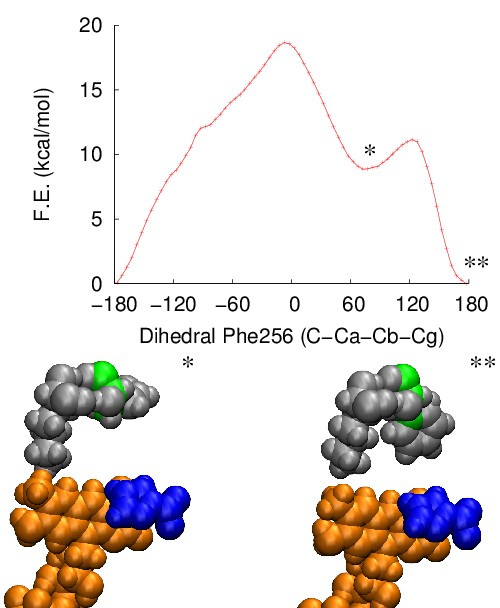
\includegraphics[width=0.5\textwidth]{msox_ph256_gate}}
+(0,-6.5) node(text1) [anchor=north west,text width=0.5\textwidth] {Substrate induces closure of Phe256 ``gate''.}
++(6.0,-1) node(image2) [graphics,anchor=north west] {
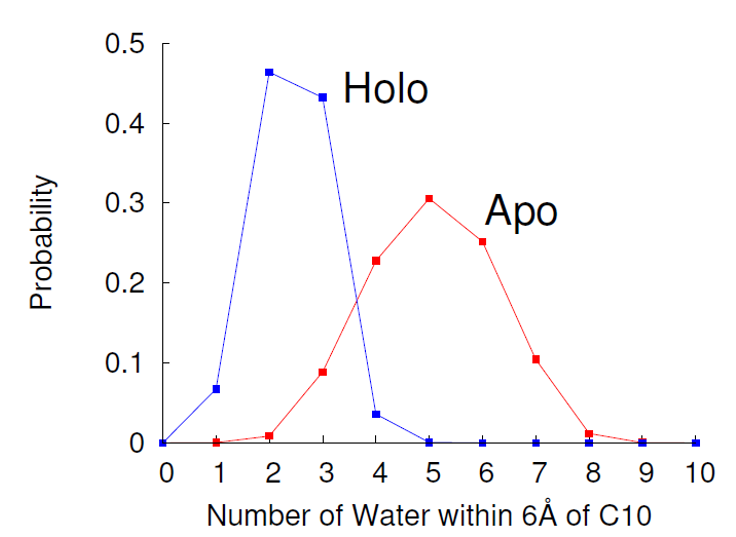
\includegraphics[width=0.5\textwidth]{msox_water}}
+(0,-4) node(text2) [anchor=north west,text width=0.5\textwidth] {Substrate pushes waters out of active site.};
\end{tikzpicture}
\end{frame}
